\documentclass[11pt]{article}

\usepackage[a4paper,margin=1in]{geometry}
\usepackage[T1]{fontenc}
\usepackage[utf8]{inputenc}
\usepackage{amsmath,amssymb}
\usepackage{graphicx}
\usepackage{booktabs}
\usepackage{multirow}
\usepackage[protrusion=true,expansion=false]{microtype}
\usepackage{xcolor}
\usepackage[font=small,labelfont=bf]{caption}
\usepackage{enumitem}
\usepackage{lmodern}
\PassOptionsToPackage{hidelinks,breaklinks}{hyperref}
\usepackage{orcidlink}
\usepackage[numbers,sort&compress]{natbib}
\usepackage{hyperref}
\usepackage{xurl}   % allow long reference URLs to break anywhere

\graphicspath{{figures/}}
% Long file paths and tied numeric expressions leave a few unbreakable boxes;
% give TeX room rather than hyphenating identifiers.
\emergencystretch=3em
\hyphenpenalty=1000
% AUTO-GENERATED by src/06_tables.py -- do not edit.
\newcommand{\secomRuns}{1{,}567}
\newcommand{\secomSignalsRaw}{590}
\newcommand{\secomSignals}{446}
\newcommand{\secomFail}{104}
\newcommand{\secomFailRate}{6.64}
\newcommand{\secomSpanDays}{89}
\newcommand{\secomMissingPct}{4.54}
\newcommand{\secomMaxColMissingPct}{91.2}
\newcommand{\secomConstantCols}{116}
\newcommand{\recallRecords}{17{,}898}
\newcommand{\recallCoveragePct}{92.2}
\newcommand{\recallExport}{2026-08-27}
\newcommand{\recallSterilityPct}{41.1}
\newcommand{\recallClassOnePct}{9.7}
\newcommand{\simBatches}{2{,}000}
\newcommand{\simFeatures}{136}
\newcommand{\simDurationH}{230}
\newcommand{\simSampleH}{2}
\newcommand{\simInjected}{131}
\newcommand{\simRejected}{147}
\newcommand{\simRejectRatePct}{7.35}
\newcommand{\simObservableFail}{121}
\newcommand{\simUnobservableFail}{10}
\newcommand{\simSpecPercentile}{0.27}
\newcommand{\simSpecCalBatches}{500}
\newcommand{\monAlpha}{0.010}
\newcommand{\monFA}{0.070\,$\pm$\,0.028}
\newcommand{\monFAfold}{7}
\newcommand{\monDetObs}{0.673\,$\pm$\,0.066}
\newcommand{\monDetUnobs}{0.136\,$\pm$\,0.159}
\newcommand{\monTTD}{136\,$\pm$\,11}
\newcommand{\monNObsFail}{39}
\newcommand{\monNUnobsFail}{4}
\newcommand{\readyAUROC}{0.799\,$\pm$\,0.029}
\newcommand{\readyAUPRC}{0.612\,$\pm$\,0.044}
\newcommand{\readyPrev}{0.074}
\newcommand{\readyLift}{8.3\,$\pm$\,0.6}
\newcommand{\nSeeds}{10}
\newcommand{\nMethods}{6}
\newcommand{\agreeCtstRho}{0.60}
\newcommand{\agreeCtstP}{0.21}
\newcommand{\agreeKsRho}{1.00}
\newcommand{\agreeKsP}{0.00}
\newcommand{\agreeCorrRho}{0.89}
\newcommand{\agreeCorrP}{0.02}
\newcommand{\agreePcaRho}{0.77}
\newcommand{\agreePcaP}{0.07}
\newcommand{\agreeAurocRho}{0.09}
\newcommand{\agreeAurocP}{0.87}
\newcommand{\agreeAuprcRho}{0.31}
\newcommand{\agreeAuprcP}{0.54}
\newcommand{\agreeDcrRho}{1.00}
\newcommand{\agreeDcrP}{0.00}
\newcommand{\agreeMiaRho}{0.66}
\newcommand{\agreeMiaP}{0.16}
\newcommand{\ciCtstRho}{0.68\,$\pm$\,0.11}
\newcommand{\ciCtstLo}{0.50}
\newcommand{\ciCtstHi}{0.82}
\newcommand{\sepCtstSim}{14.0}
\newcommand{\sepCtstReal}{5.5}
\newcommand{\ciKsRho}{0.97\,$\pm$\,0.04}
\newcommand{\ciKsLo}{0.91}
\newcommand{\ciKsHi}{1.00}
\newcommand{\sepKsSim}{17.8}
\newcommand{\sepKsReal}{22.6}
\newcommand{\ciCorrRho}{0.88\,$\pm$\,0.04}
\newcommand{\ciCorrLo}{0.82}
\newcommand{\ciCorrHi}{0.92}
\newcommand{\sepCorrSim}{18.2}
\newcommand{\sepCorrReal}{6.9}
\newcommand{\ciPcaRho}{0.71\,$\pm$\,0.14}
\newcommand{\ciPcaLo}{0.49}
\newcommand{\ciPcaHi}{0.83}
\newcommand{\sepPcaSim}{12.6}
\newcommand{\sepPcaReal}{6.3}
\newcommand{\ciAurocRho}{0.09\,$\pm$\,0.31}
\newcommand{\ciAurocLo}{-0.13}
\newcommand{\ciAurocHi}{0.47}
\newcommand{\sepAurocSim}{2.1}
\newcommand{\sepAurocReal}{0.7}
\newcommand{\ciAuprcRho}{0.14\,$\pm$\,0.35}
\newcommand{\ciAuprcLo}{-0.09}
\newcommand{\ciAuprcHi}{0.57}
\newcommand{\sepAuprcSim}{2.2}
\newcommand{\sepAuprcReal}{0.6}
\newcommand{\ciDcrRho}{0.88\,$\pm$\,0.08}
\newcommand{\ciDcrLo}{0.77}
\newcommand{\ciDcrHi}{0.97}
\newcommand{\sepDcrSim}{2.6}
\newcommand{\sepDcrReal}{1.8}
\newcommand{\ciMiaRho}{0.55\,$\pm$\,0.22}
\newcommand{\ciMiaLo}{0.24}
\newcommand{\ciMiaHi}{0.80}
\newcommand{\sepMiaSim}{1.1}
\newcommand{\sepMiaReal}{1.5}
\newcommand{\ciFidPrivLo}{0.55}
\newcommand{\ciFidPrivHi}{0.97}
\newcommand{\ciUtilLo}{0.09}
\newcommand{\ciUtilHi}{0.14}
\newcommand{\ciContrastMedFid}{0.83}
\newcommand{\ciContrastMedUtil}{-0.03}
\newcommand{\ciContrastP}{<0.001}
\newcommand{\ciNFidPriv}{60}
\newcommand{\ciNUtil}{8}
\newcommand{\agreeMedianRho}{0.71}
\newcommand{\agreeNMetrics}{8}
\newcommand{\agreeFidPrivMin}{0.60}
\newcommand{\agreeFidPrivMax}{1.00}
\newcommand{\agreeFidPrivN}{6}
\newcommand{\agreeUtilMax}{0.31}
\newcommand{\agreeNSignif}{3}
\newcommand{\bootDcrReal}{0.000\,$\pm$\,0.000}
\newcommand{\bootMiaReal}{0.813\,$\pm$\,0.016}
\newcommand{\bootCopyReal}{0.593\,$\pm$\,0.029}
\newcommand{\bootCtstReal}{0.308\,$\pm$\,0.024}
\newcommand{\trtrAuprcReal}{0.157\,$\pm$\,0.022}
\newcommand{\trtrAurocReal}{0.682\,$\pm$\,0.029}
\newcommand{\prevReal}{0.066}
\newcommand{\trtrAuprcSim}{0.893\,$\pm$\,0.037}
\newcommand{\trtrAurocSim}{0.975\,$\pm$\,0.012}
\newcommand{\prevSim}{0.074}
\newcommand{\bestCtstReal}{copula}
\newcommand{\bestCtstRealVal}{0.957\,$\pm$\,0.018}
\newcommand{\bestCtstSim}{copula}
\newcommand{\bestCtstSimVal}{0.841\,$\pm$\,0.027}
\newcommand{\bestCorrReal}{gaussian}
\newcommand{\bestCorrRealVal}{0.037\,$\pm$\,0.001}
\newcommand{\bestCorrSim}{gaussian}
\newcommand{\bestCorrSimVal}{0.025\,$\pm$\,0.002}
\newcommand{\bestUtilReal}{vae}
\newcommand{\bestUtilRealVal}{0.116\,$\pm$\,0.048}
\newcommand{\bestUtilSim}{gmm}
\newcommand{\bestUtilSimVal}{0.613\,$\pm$\,0.069}
\newcommand{\bestPcaReal}{gaussian}
\newcommand{\bestPcaRealVal}{0.781\,$\pm$\,0.024}
\newcommand{\bestPcaSim}{gaussian}
\newcommand{\bestPcaSimVal}{0.890\,$\pm$\,0.028}
\newcommand{\bestUtilRetainReal}{0.74}
\newcommand{\bestUtilRetainSim}{0.69}
\newcommand{\sprMarginalReal}{0.0664}
\newcommand{\sprRatioMarginalReal}{1.00}
\newcommand{\sprGaussianReal}{0.2602}
\newcommand{\sprRatioGaussianReal}{3.92}
\newcommand{\sprCopulaReal}{0.0628}
\newcommand{\sprRatioCopulaReal}{0.95}
\newcommand{\sprGmmReal}{0.0494}
\newcommand{\sprRatioGmmReal}{0.74}
\newcommand{\sprVaeReal}{0.0013}
\newcommand{\sprRatioVaeReal}{0.02}
\newcommand{\sprWganReal}{0.0063}
\newcommand{\sprRatioWganReal}{0.09}
\newcommand{\sprMarginalSim}{0.0695}
\newcommand{\sprRatioMarginalSim}{0.94}
\newcommand{\sprGaussianSim}{0.0848}
\newcommand{\sprRatioGaussianSim}{1.15}
\newcommand{\sprCopulaSim}{0.0742}
\newcommand{\sprRatioCopulaSim}{1.01}
\newcommand{\sprGmmSim}{0.0598}
\newcommand{\sprRatioGmmSim}{0.81}
\newcommand{\sprVaeSim}{0.0065}
\newcommand{\sprRatioVaeSim}{0.09}
\newcommand{\sprWganSim}{0.0358}
\newcommand{\sprRatioWganSim}{0.49}
\newcommand{\vaeDegenRealPct}{60}
\newcommand{\vaeDegenRealSeeds}{4}


\newcommand{\corpusreal}{SECOM}

\title{\textbf{Circular by Construction:\\ What Synthetic Process-Data Generators
Can and Cannot Establish\\ for Batch Release}}

\author{Phani Kumar Balagam\,\orcidlink{0009-0007-6762-399X}\\
\small Independent Researcher\\
\small \texttt{balagam.phani@gmail.com}}

\date{\today}

\begin{document}
\maketitle

\begin{abstract}
\noindent
Synthetic ``digital twins'' of batch manufacturing are almost always validated
against the simulator that produced their training data. That practice
supports some conclusions and not the one that matters. We build a two-layer
open benchmark separating the ground-truth process from the learned
twin---a mechanistic fed-batch simulator whose failure-mode prior is anchored to
\recallRecords{} FDA drug-recall records, and \nMethods{} generative models
trained on its output---and run one protocol on both corpora. No \emph{pharmaceutical} batch records are public, so
the real corpus is \corpusreal{} (\secomRuns{} semiconductor production runs,
\secomSignals{} signals, \secomFailRate{}\% failing), a structural stand-in.
Fidelity and privacy conclusions transfer: over \agreeFidPrivN{} such metrics
the per-seed rank correlation between corpora is
$\rho \in [\ciFidPrivLo{}, \ciFidPrivHi{}]$. Utility conclusions do not
($\rho$~=~\ciAurocRho{} for transfer AUROC, \ciAuprcRho{} for AUPRC; both
intervals span zero). Absolute utility does not carry over either: at comparable
prevalence the simulated task is far easier (train-on-real AUPRC
\trtrAuprcSim{} against \trtrAuprcReal{}). That gap belongs to \emph{this}
simulator, whose disposition label is near-deterministic in its own trajectory;
a builder without real batch records cannot know its size or sign.
Generators emit failing real batches at
\sprRatioVaeReal{}$\times$ to \sprRatioGaussianReal{}$\times$ the true rate
while aggregate fidelity barely registers it, and trajectory monitoring detects
\monDetObs{} of failures leaving a process signature against \monDetUnobs{} of
those that do not. We offer a benchmark and a protocol, not a release-decision
system, and say which parts stay with the quality unit.
\end{abstract}

\vspace{0.5em}
\noindent\fbox{\parbox{0.97\linewidth}{\footnotesize
This work was carried out independently, on personal time and equipment, and is
not connected to the author's employment. The views expressed are the author's
own and do not represent the views, positions or policies of any current, former
or future employer or client. No proprietary, confidential or internal data of
any organization was used. All data is public: the SECOM dataset from the UCI
Machine Learning Repository, the openFDA drug enforcement (recall) bulk export,
and a simulated corpus generated by the code released with this paper.}}

\section{Introduction}

A ``digital twin'' of a pharmaceutical manufacturing process is usually proposed
with two applications in view: detecting abnormal process trajectories while a
batch is running, and anticipating whether the batch will meet its
specifications at release. Both are attractive, and both run into the same
obstacle. Real GMP batch records are among the most tightly held data in the
industry. There is no public corpus of them. Every openly reproducible study of
batch monitoring or release prediction therefore works on simulated data.

That constraint is usually acknowledged and then treated as a nuisance. We argue
it is the central methodological problem, and that its consequences are
measurable. When a generative model is trained on simulator output and then
scored against further simulator output, the evaluation is closed: it establishes
that the model learned the simulator, and says nothing about the process the
simulator was meant to stand for. The literature on synthetic tabular data has
developed careful fidelity and utility metrics~\citep{alaa2022faithful}, and has
learned to test privacy claims rather than assume
them~\citep{stadler2022synthetic}; but every one of those measures inherits
whatever reference distribution it is given. Applied inside a closed loop they
report high scores that mean nothing about reality.

The question we can actually answer with public data is narrower than
``is the simulator realistic?'' --- which is unanswerable without real batch
records --- but it is not vacuous. It is: \emph{do conclusions drawn from
evaluating generators on simulated process data transfer to real process data?}
Our answer turns out to depend on which conclusion. Judgements about how well a
generator reproduces a distribution, and about whether it memorises its training
records, transfer well. Judgements about whether the synthetic data is any
\emph{use} downstream do not transfer at all --- and that is the judgment on
which a release-support application would rest.

\paragraph{Contributions.}
\begin{enumerate}[leftmargin=1.4em,itemsep=1pt,topsep=2pt]
\item We state the circularity problem in digital-twin evaluation for batch
release precisely, and give a two-layer benchmark design (Figure~\ref{fig:design})
that separates the ground-truth process from the learned twin so that the
circularity is visible rather than implicit (\S\ref{sec:circular}, \S\ref{sec:bench}).
\item We release a mechanistic fed-batch simulator whose failure-mode prior is
anchored to real data: \recallRecords{} FDA drug-recall records
(\recallCoveragePct{}\% classified by an auditable rule set), of which the
process-relevant subset is renormalized into the simulator's fault model
(\S\ref{sec:sim}). Two of its six failure modes deliberately leave no trajectory
signature, so detection has a principled ceiling rather than an artificial one.
\item We run one identical fidelity/utility/privacy protocol on a real
manufacturing corpus and on the simulated corpus, over \nSeeds{} seeds, and
report the agreement between them as the primary result: fidelity and privacy
rankings transfer, utility rankings do not, and absolute utility levels are not
comparable at all (\S\ref{sec:transfer}).
\item We report the negative results rather than the best operating point:
generators that reproduce the process well and the \emph{failures} badly, a
detection ceiling set by failure modes the instrumentation cannot see, and
false-alarm inflation of roughly \monFAfold{}-fold from testing repeatedly along
a batch --- the last two measured on the simulated corpus only, for want of any
real trajectories (\S\ref{sec:results}).
\item We state the decision-support boundary explicitly: what a system of this
kind could contribute to a release workflow, what stays with the quality unit,
and what a qualification path would require before any of it could be used
(\S\ref{sec:regulatory}).
\end{enumerate}

We do not claim a release-readiness system. We claim a benchmark, a protocol, and
evidence that the current evaluation practice does not support the claims made
with it.

\begin{figure}[t]
\centering
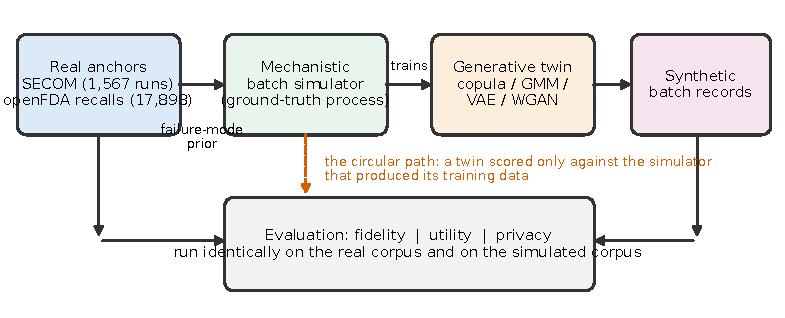
\includegraphics[width=\linewidth]{fig1_design.pdf}
\caption{The two-layer benchmark. A mechanistic simulator plays the role of the
ground-truth process; generative models play the role of the digital twin. The
dashed red path is the circular evaluation this paper is about: a twin scored
only against the simulator that produced its training data. The horizontal path
is what we do instead --- one evaluation protocol applied identically to the
simulated corpus and to a real manufacturing corpus, so that the two answers can
be compared.}
\label{fig:design}
\end{figure}

\section{Batch release is not a prediction problem}
\label{sec:regulatory-background}

It is worth being precise about the act this work is adjacent to, because the
imprecision is common and it matters for what may be claimed.

In the United States, \S211.22 of 21~CFR Part~211 vests in the quality control
unit the responsibility and authority to approve or reject all components, drug
product containers, closures, in-process materials, packaging material, labeling
and drug products. \S211.192 then requires that all drug product production and
control records be reviewed \emph{and approved by that unit} before a batch is
released or distributed, and that any unexplained discrepancy or failure of a
batch to meet its specifications be thoroughly investigated --- notably,
\emph{whether or not the batch has already been distributed}~\citep{cfr211}. In the European Union
the corresponding act is certification by a Qualified Person under EudraLex
Volume~4 Annex~16, which places personal responsibility on a named individual for
confirming that each batch was manufactured and checked in compliance with the
marketing authorisation and with GMP~\citep{eudralex2015annex16}. The two regimes
differ in whom they name, but agree on the essential point: release is a
documented human decision with an accountable owner, taken on a complete batch
record, not an inference.

Nothing in this paper changes that, and no result below should be read as
progress toward changing it. A model cannot hold the authority that
\S211.22 assigns or sign the certification Annex~16 requires. What a model can
do is order work, focus attention, and flag records for review earlier than they
would otherwise be seen. We return to exactly which of those is supported by our
evidence in \S\ref{sec:regulatory}.

\section{The circularity problem}
\label{sec:circular}

Let $\mathcal{P}$ denote the real process distribution over batch records, and
$\mathcal{S}$ a simulator intended to approximate it. A generative twin $G$ is
fitted to a sample $D \sim \mathcal{S}$ and produces synthetic records
$\hat{D} \sim G$. The standard evaluation reports a divergence
$d(\hat{D}, D')$ for a further $D' \sim \mathcal{S}$.

Two distinct quantities are being conflated. The reported $d(\hat{D}, D')$ bounds
how well $G$ learned $\mathcal{S}$. The quantity of interest is
$d(\hat{D}, \mathcal{P})$, which by the triangle inequality is bounded below by
$d(\mathcal{S}, \mathcal{P}) - d(\hat{D}, \mathcal{S})$. The term
$d(\mathcal{S},\mathcal{P})$ --- simulator realism --- is never estimated,
because estimating it requires the real batch records whose absence motivated the
simulator in the first place. It is not small by assumption, and no amount of
improvement in $d(\hat{D},\mathcal{S})$ constrains it. A twin can be arbitrarily
good at reproducing a simulator that is arbitrarily wrong.

This is why we do not attempt to argue that our simulator is realistic. We
instead test a weaker but checkable proposition. Write $\mathcal{R}$ for a real
process distribution from which we do have a sample. If a metric's ranking of
generators computed under $\mathcal{S}$ agreed with its ranking under
$\mathcal{R}$, then simulator-based evaluation would at least be a useful proxy
for method selection, whatever its absolute bias. If the rankings disagree, the
proxy fails on its own terms. \S\ref{sec:transfer} measures that agreement.

\section{Benchmark}
\label{sec:bench}

\subsection{Real anchors}
\label{sec:anchors}

No public corpus of real pharmaceutical batch records exists, so we use two real
corpora that are each partial substitutes, and we are explicit about which
question each can and cannot answer.

\paragraph{\corpusreal{}: real process data with real disposition labels.}
The SECOM dataset~\citep{mccann2008secom} contains \secomRuns{} production runs
from a semiconductor fabrication line, each with \secomSignalsRaw{} sensor
measurements and a pass/fail disposition, collected over \secomSpanDays{} days.
\secomFail{} runs (\secomFailRate{}\%) failed. The corpus has the pathologies of
real plant data: \secomMissingPct{}\% of cells are missing, one signal is missing
in \secomMaxColMissingPct{}\% of runs, and \secomConstantCols{} signals are
constant. After dropping constant and mostly-missing signals and median-imputing
the rest, \secomSignals{} signals remain. It is not pharmaceutical. It \emph{is}
a real, high-dimensional, weakly-labelled manufacturing process with a rare
failure class and a genuine disposition decision attached, which is the
structure our protocol needs. We use it to ask whether conclusions transfer, not
to claim pharmaceutical relevance.

\paragraph{openFDA recalls: a real prior over failure modes.}
We use the openFDA drug enforcement corpus (export \recallExport{}) to anchor
\emph{which} failures occur and how severe they are.
\recallRecords{} drug recall records were classified into manufacturing failure
modes by an ordered regular-expression rule set;
\recallCoveragePct{}\% matched a rule and the remainder are reported as
unclassified rather than forced. Microbial and sterility failures dominate at
\recallSterilityPct{}\% of records, and \recallClassOnePct{}\% of all records are
Class~I. Figure~\ref{fig:prior} shows the empirical distribution and the
renormalization into the simulator's fault model.

This anchor has a bias that must be stated: recall records describe failures that
\emph{escaped} release and were detected in the market. Modes that batch release
reliably catches are systematically under-represented. The corpus therefore
constrains the failure-mode \emph{mix} of the simulator; it cannot estimate a
batch rejection rate, and we do not use it for one.

\begin{figure}[t]
\centering
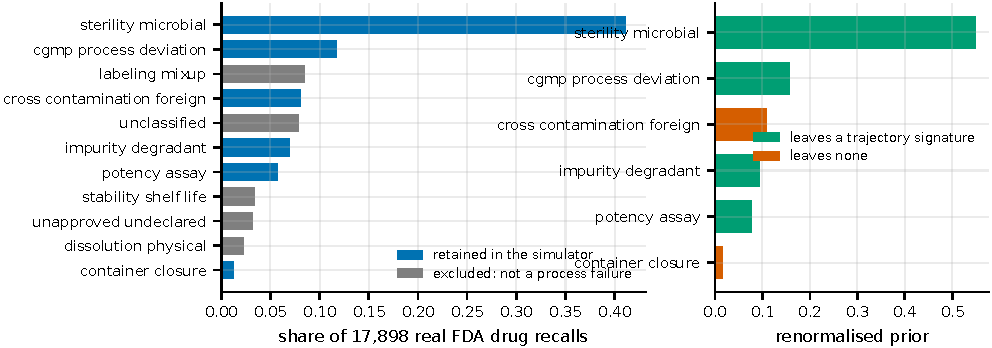
\includegraphics[width=\linewidth]{fig2_failure_prior.pdf}
\caption{Left: empirical failure-mode distribution over \recallRecords{} real FDA
drug recall records. Modes that are not bioreactor process failures (labeling
mix-ups, regulatory status, shelf-life, solid-dose attributes) and unclassified
records are excluded. Right: the retained modes after renormalization, colored
by whether the mode leaves a signature in the process trajectory. The two red
modes set a hard ceiling on what any trajectory-based monitor can detect.}
\label{fig:prior}
\end{figure}

\subsection{Mechanistic simulator}
\label{sec:sim}

The ground-truth process layer is a fed-batch fermentation model in the
Bajpai--Reuss tradition~\citep{bajpai1980mechanistic}, of the kind used in the
PenSim~\citep{birol2002modular} and industrial-scale
IndPenSim~\citep{goldrick2015development,goldrick2019modern} benchmarks. Biomass,
substrate and product follow Monod kinetics with dissolved-oxygen, pH and
temperature dependence; production uses a lower half-saturation constant with
substrate inhibition, so the process keeps producing under the substrate-limited
regime it is deliberately operated in. Feed is exponential during the production
phase; pH, temperature and dissolved oxygen are held by PI controllers with
actuator noise. Seventeen process parameters vary batch to batch with stated
coefficients of variation, representing seed-train and raw-material variability;
Appendix~\ref{app:calibration} lists what they cover and how they were set.

Each batch runs \simDurationH{}~h and is sampled every \simSampleH{}~h across
eight process variables, then passed through a sensor layer that adds
measurement noise, a per-batch linear drift, and random dropouts. Batches are
summarized into a \simFeatures{}-feature batch record: phase-wise mean, standard
deviation, minimum and maximum of every variable over four process phases, plus
eight release CQAs.

\paragraph{Failure modes and the observability ceiling.}
Six failure modes are injected with the renormalized recall prior. Four leave a
trajectory signature (microbial contamination, chronic under-production, a
thermal excursion driving degradant formation, a controlled-parameter deviation).
Two do not: foreign particulate contamination and a container-closure defect
arise after or outside the process the sensors observe. This is deliberate. A
benchmark in which every fault is detectable rewards models for solving a problem
that does not exist, and hides the fact that trajectory monitoring has a real
upper bound set by what the instrumentation can see.

\paragraph{What this simulator does and does not claim.}
We make no realism claim for the simulator, and we avoid the word faithful,
because as commonly used it admits no test. What can be checked about this model
is its provenance and the behavior its equations entail: the model form is the
published fed-batch structure cited above; production continues under
substrate limitation with inhibition at high substrate; a competing organism
depletes dissolved oxygen and substrate before product titer falls
(Figure~\ref{fig:traj}); and a thermal excursion raises degradant through the
hydrolysis term. Those are refusable statements about this model, and a reader
who finds the trajectories inconsistent with them has found an error. Nothing
beyond them is asserted: no parameter was fitted to plant data, the absolute
titer scale is arbitrary, and the model is best read as a parameterised
data-generating process rather than a representation of any plant.
Appendix~\ref{app:calibration} records how its parameters were set.
We therefore do not assert real product specifications. Limits are derived from the
simulator's own nominal distribution over \simSpecCalBatches{} fault-free
batches, at the \simSpecPercentile{}th and complementary percentile
($\pm 3\sigma$ equivalent). This is a direct consequence of having no real batch
data to calibrate against, and it is exactly the kind of unfalsifiable modeling
choice this paper is warning about; we make it visible rather than bury it.

Over \simBatches{} batches, \simInjected{} received an injected fault and
\simRejected{} (\simRejectRatePct{}\%) fell out of specification, of which
\simObservableFail{} had an observable mode and \simUnobservableFail{} did not.
The nominal batch failure rate was set to match \corpusreal{}'s observed failure
rate so the two corpora are comparable in class balance; this is an assumption,
not an estimate. Figure~\ref{fig:traj} shows nominal and contaminated
trajectories.

\begin{figure}[t]
\centering
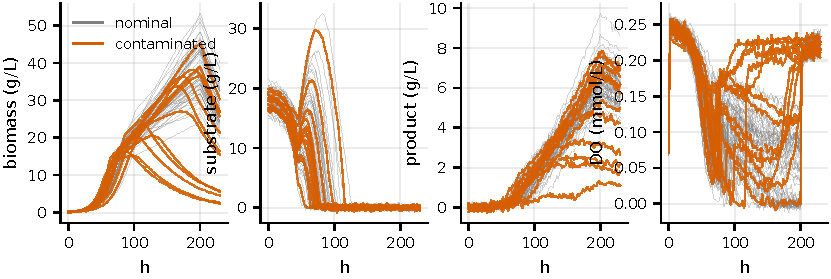
\includegraphics[width=\linewidth]{fig3_trajectories.pdf}
\caption{Simulated process trajectories: 60 nominal batches (grey) and 12 batches
with microbial contamination (red). Contamination competes for substrate and
oxygen, so its signature appears in dissolved oxygen and substrate before it
appears in product titer --- which is what makes early detection possible for
this mode and impossible for the two modes that leave no trajectory signature at
all.}
\label{fig:traj}
\end{figure}

\section{Generators and evaluation protocol}
\label{sec:protocol}

\subsection{Generators}
We compare \nMethods{} generators spanning the families a synthetic-tabular-data
study is expected to cover: an independence baseline that reproduces every
marginal exactly and destroys all dependence; a shrinkage multivariate
Gaussian~\citep{ledoit2004wellconditioned}; a Gaussian copula with
non-parametric margins; a diagonal Gaussian mixture with components chosen by
BIC; an MLP variational autoencoder~\citep{kingma2014autoencoding}; and a
Wasserstein GAN with gradient penalty~\citep{gulrajani2017improved}, standing in
for the CTGAN family~\citep{xu2019modeling} without its categorical machinery,
which this all-continuous setting does not require.

We additionally report \emph{bootstrap resampling} of the training rows. This is
not a method under evaluation. It is a reference point that is perfect on
fidelity and utility and maximally bad on privacy, included so that the trade-off
between the three axes is visible in the same table rather than asserted.

The disposition label is modelled jointly with the features, as a batch-record
generator would have to, and thresholded at $0.5$ when sampled.

\paragraph{Budgets.} Reported so that a reader can judge whether a result is a
property of a method or of its training budget. The VAE uses latent~32, two
hidden layers of 256, 250 epochs, Adam at $10^{-3}$, batch 128, with KL warm-up
over the first 30\% of epochs. The WGAN-GP uses latent~64, hidden 256, 1{,}200
generator steps, 3 critic steps per generator step, Adam at $2\times10^{-4}$,
batch 128, gradient penalty 10. The Gaussian mixture selects $k \in \{2,4,8\}$ by
BIC with diagonal covariance. The classifier two-sample test uses 3-fold
cross-validated gradient boosting (150 iterations); the downstream classifier
uses 200. Synthetic samples are drawn at $1\times$ the training-set size for
fidelity and privacy and $5\times$ for utility. No per-corpus hyperparameter
search was performed: the same budget is used on both corpora and for every
seed.

\subsection{Protocol}
Each corpus is split into three disjoint halves-of-halves: a training set that
fits the generator, a holdout that serves as the non-member set for privacy
tests, and a test set used only for utility. No set serves two purposes.
Per-generator results are reported as mean\,$\pm$\,standard deviation over
\nSeeds{} seeds; rank correlations additionally carry a 5--95\% percentile
interval over the same seeds. No single-run number appears in this paper.

\paragraph{Fidelity.} Per-column two-sample Kolmogorov--Smirnov statistics and
Wasserstein distances for marginals; mean absolute difference of the Pearson and
Spearman correlation matrices and top-10 PCA subspace overlap for joints; and a
classifier two-sample test~\citep{lopezpaz2017revisiting}, cross-validated,
where AUC $0.5$ means indistinguishable.

\paragraph{Utility.} Train-on-synthetic, test-on-real: a gradient-boosted
classifier is fitted on synthetic records and evaluated on the held-out real test
set, against a train-real/test-real baseline. Because the failing class is rare,
we draw five times the training-set size of synthetic records before fitting. A
generator that still yields fewer than five failing records has failed to
represent the minority class, and we report that outcome rather than working
around it.

\paragraph{Privacy.} Distance to closest record is reported as a \emph{ratio} of
median distance-to-training over median distance-to-holdout: a generator that
merely produces typical records sits close to everything, so the absolute
distance is uninformative and the ratio is not. A ratio near $1$ means the
generator is no closer to its training data than to unseen data of the same kind.
We also report the nearest-neighbour distance ratio, the exact-copy fraction, and
a membership inference attack in the sense of \citet{shokri2017membership},
implemented here as a nearest-neighbour distance attack rather than their
shadow-model classifier, and scored by AUC over training members versus holdout
non-members.

\section{Results}
\label{sec:results}

\paragraph{What we expected, and what we found.} We state this before the
numbers because it bears on how they should be read. The study was designed
expecting that generator rankings would fail to transfer across the board, and
the first draft of this paper asserted exactly that. They did not: fidelity and
privacy rankings transfer well, and only utility fails. The framing in
\S\ref{sec:transfer} was rewritten around that split after the results were in.
No metric, generator or corpus was added or dropped in response to the outcome,
and the analysis was run once over the ten seeds fixed in advance; but the
\emph{interpretation} is post hoc and we do not present it as a preregistered
prediction. The simulator itself went through several calibration passes before
any evaluation was run --- kinetic parameters and the feed profile were adjusted
until nominal titer and reject rate were plausible, and the specification limits
were changed from asserted values to percentiles of the simulator's own nominal
distribution after the asserted values rejected every batch
(\S\ref{sec:sim}). The neural budgets were also cut once for runtime, before the reported runs and
applied uniformly thereafter: the WGAN from 3{,}000 to 1{,}200 generator steps
and from five critic steps to three, the VAE from 400 to 250 epochs, and the
classifier two-sample test from five folds to three. Both sequences are modeling
history, not results, and they are disclosed here because a paper about
undisclosed evaluation choices should not have any. \S\ref{sec:limitations}
returns to what the reduced budgets may cost the neural generators.

\subsection{Generator behavior on each corpus}

Table~\ref{tab:main} gives the full protocol on both corpora. Three patterns hold
across both.

First, the classifier two-sample test saturates. On both corpora, most generators
are separated from real data with AUC indistinguishable from $1.0$: in several
hundred dimensions with one to two thousand rows, a gradient-boosted classifier
finds a discriminating direction for nearly any generator. C2ST is the metric a
generative-modeling reviewer will look for, and on data of this shape it is
close to useless for ranking. We report it because its saturation is itself a
result about evaluating synthetic manufacturing data, not because it separates
methods.

Second, marginal fidelity and joint fidelity come apart sharply. The independence
baseline reproduces every marginal essentially exactly --- by construction --- and
is among the best generators on mean KS while being the worst possible model of
the joint distribution. Any evaluation that leads on marginal agreement will
rank a model that has learned nothing about the process at the top.

Third, the bootstrap reference behaves as designed and makes the privacy axis
legible: DCR ratio \bootDcrReal{} and membership-inference AUC \bootMiaReal{} on
the real corpus, with an exact-copy fraction of \bootCopyReal{}. It is the best
available generator on utility and offers no privacy at all. Every other row in
the table should be read against it. Its C2ST AUC of \bootCtstReal{} falls
\emph{below} chance, which is an artefact worth naming: because bootstrap
duplicates training rows, the same record appears in both classes, and a
classifier that memorises it in training is systematically wrong on it in
validation.

On the metrics that do separate methods, the two corpora agree on the winner
more often than not. The Gaussian copula is the only generator the C2ST cannot
saturate on either corpus (\bestCtstRealVal{} real, \bestCtstSimVal{}
simulated), and the shrinkage Gaussian gives the best joint structure on both
(correlation MAE \bestCorrRealVal{} real, \bestCorrSimVal{} simulated). It is on
the third axis that the agreement breaks down.

\begin{table}[t]
\centering
\scriptsize
\setlength{\tabcolsep}{3.5pt}
\caption{Fidelity, utility and privacy on both corpora, mean\,$\pm$\,sd over
\nSeeds{} seeds. C2ST AUC $0.5$ is ideal; the bootstrap row's sub-chance C2ST is
the duplicate-record artefact explained in \S\ref{sec:results} and is not
comparable with the others. KS and correlation MAE lower is better;
PCA overlap and TSTR AUPRC higher is better; DCR ratio $1$ means no memorisation
and MIA AUC $0.5$ means the attack learns nothing. $^\dagger$Bootstrap is a
reference point, not a method: it copies training rows.}
\label{tab:main}
\resizebox{\linewidth}{!}{% AUTO-GENERATED by src/06_tables.py -- do not edit.
\begin{tabular}{llcccccccc}
\toprule
corpus & generator & C2ST AUC & KS & corr MAE & PCA ovl & TSTR AUROC & TSTR AUPRC & DCR ratio & MIA AUC \\
\midrule
SECOM (real) & \textit{bootstrap}$^\dagger$ & 0.308\,$\pm$\,0.024 & 0.029\,$\pm$\,0.001 & 0.028\,$\pm$\,0.003 & 0.717\,$\pm$\,0.038 & 0.661\,$\pm$\,0.044 & 0.145\,$\pm$\,0.030 & 0.000\,$\pm$\,0.000 & 0.813\,$\pm$\,0.016 \\
 & marginal & 1.000\,$\pm$\,0.000 & 0.029\,$\pm$\,0.000 & 0.059\,$\pm$\,0.001 & 0.028\,$\pm$\,0.005 & 0.468\,$\pm$\,0.038 & 0.069\,$\pm$\,0.016 & 0.992\,$\pm$\,0.007 & 0.514\,$\pm$\,0.017 \\
 & gaussian & 1.000\,$\pm$\,0.000 & 0.190\,$\pm$\,0.005 & 0.037\,$\pm$\,0.001 & 0.781\,$\pm$\,0.024 & 0.533\,$\pm$\,0.066 & 0.089\,$\pm$\,0.025 & 0.986\,$\pm$\,0.004 & 0.531\,$\pm$\,0.018 \\
 & copula & 0.957\,$\pm$\,0.018 & 0.030\,$\pm$\,0.000 & 0.044\,$\pm$\,0.001 & 0.465\,$\pm$\,0.038 & 0.554\,$\pm$\,0.044 & 0.106\,$\pm$\,0.024 & 0.980\,$\pm$\,0.005 & 0.529\,$\pm$\,0.016 \\
 & gmm & 1.000\,$\pm$\,0.000 & 0.132\,$\pm$\,0.004 & 0.049\,$\pm$\,0.004 & 0.391\,$\pm$\,0.089 & 0.534\,$\pm$\,0.052 & 0.092\,$\pm$\,0.026 & 0.986\,$\pm$\,0.005 & 0.520\,$\pm$\,0.021 \\
 & vae & 1.000\,$\pm$\,0.000 & 0.192\,$\pm$\,0.005 & 0.054\,$\pm$\,0.001 & 0.470\,$\pm$\,0.048 & 0.563\,$\pm$\,0.057 & 0.116\,$\pm$\,0.048 & 0.961\,$\pm$\,0.009 & 0.592\,$\pm$\,0.020 \\
 & wgan & 1.000\,$\pm$\,0.001 & 0.233\,$\pm$\,0.008 & 0.068\,$\pm$\,0.001 & 0.608\,$\pm$\,0.036 & 0.566\,$\pm$\,0.074 & 0.099\,$\pm$\,0.019 & 0.975\,$\pm$\,0.006 & 0.539\,$\pm$\,0.018 \\
\midrule
simulated & \textit{bootstrap}$^\dagger$ & 0.305\,$\pm$\,0.012 & 0.028\,$\pm$\,0.002 & 0.024\,$\pm$\,0.001 & 0.842\,$\pm$\,0.036 & 0.993\,$\pm$\,0.005 & 0.950\,$\pm$\,0.029 & 0.000\,$\pm$\,0.000 & 0.810\,$\pm$\,0.013 \\
 & marginal & 1.000\,$\pm$\,0.000 & 0.026\,$\pm$\,0.001 & 0.116\,$\pm$\,0.001 & 0.084\,$\pm$\,0.016 & 0.412\,$\pm$\,0.061 & 0.068\,$\pm$\,0.016 & 0.985\,$\pm$\,0.004 & 0.503\,$\pm$\,0.022 \\
 & gaussian & 1.000\,$\pm$\,0.000 & 0.094\,$\pm$\,0.003 & 0.025\,$\pm$\,0.002 & 0.890\,$\pm$\,0.028 & 0.780\,$\pm$\,0.060 & 0.508\,$\pm$\,0.095 & 0.972\,$\pm$\,0.005 & 0.519\,$\pm$\,0.024 \\
 & copula & 0.841\,$\pm$\,0.027 & 0.028\,$\pm$\,0.003 & 0.035\,$\pm$\,0.001 & 0.705\,$\pm$\,0.021 & 0.704\,$\pm$\,0.074 & 0.248\,$\pm$\,0.087 & 0.969\,$\pm$\,0.005 & 0.518\,$\pm$\,0.025 \\
 & gmm & 1.000\,$\pm$\,0.000 & 0.051\,$\pm$\,0.001 & 0.065\,$\pm$\,0.001 & 0.457\,$\pm$\,0.025 & 0.840\,$\pm$\,0.042 & 0.613\,$\pm$\,0.069 & 0.978\,$\pm$\,0.006 & 0.515\,$\pm$\,0.025 \\
 & vae & 1.000\,$\pm$\,0.000 & 0.104\,$\pm$\,0.002 & 0.046\,$\pm$\,0.004 & 0.699\,$\pm$\,0.021 & 0.766\,$\pm$\,0.115 & 0.512\,$\pm$\,0.177 & 0.942\,$\pm$\,0.008 & 0.579\,$\pm$\,0.023 \\
 & wgan & 1.000\,$\pm$\,0.000 & 0.162\,$\pm$\,0.008 & 0.076\,$\pm$\,0.001 & 0.603\,$\pm$\,0.021 & 0.724\,$\pm$\,0.078 & 0.330\,$\pm$\,0.108 & 0.968\,$\pm$\,0.005 & 0.512\,$\pm$\,0.026 \\
\bottomrule
\end{tabular}
}
\end{table}

\subsection{Do conclusions transfer from simulated to real data?}
\label{sec:transfer}

This is the paper's primary question. For each metric we rank the \nMethods{}
generators by their mean on the simulated corpus and by their mean on the real
corpus, and compare the two rankings. The answer splits cleanly by axis.

We report the correlation \emph{per seed}: for each seed we rank the six
generators on the simulated corpus and on the real corpus at that seed and
correlate the two rankings, giving \nSeeds{} estimates per metric rather than one
point estimate over six method means. This matters, because with $n=\nMethods{}$
a single Spearman coefficient carries no usable uncertainty and the paper's claim
is precisely a difference between coefficients.

\paragraph{Fidelity and privacy rankings transfer.} Across the \agreeFidPrivN{}
fidelity and privacy metrics the per-seed correlation lies in
$[\ciFidPrivLo{}, \ciFidPrivHi{}]$, with every 5--95\% interval clear of zero:
marginal agreement $\rho$~=~\ciKsRho{}, joint structure $\rho$~=~\ciCorrRho{},
memorisation ratio $\rho$~=~\ciDcrRho{}, and even the saturated C2ST reaching
$\rho$~=~\ciCtstRho{}. If the only question were ``which generator best
reproduces this distribution, and does it copy its training records'', evaluating
on a simulator would be a defensible proxy. That is a real and, to us,
unexpected positive result.

One qualification belongs here rather than in the limitations. Agreement is only
meaningful where the methods actually differ. Table~\ref{tab:agreement} reports,
alongside each correlation, the between-method spread divided by the seed-level
noise. For the fidelity metrics that ratio is large (\sepKsReal{} to
\sepCorrSim{}); for the privacy metrics it is much smaller (as low as
\sepMiaSim{}), meaning the privacy rankings are computed over methods that barely
differ. We would not lean on the privacy transfer result on its own.

\paragraph{Utility rankings do not transfer.} On the axis that a
release-support application would depend on, the correlation collapses to
$\rho$~=~\ciAurocRho{} for transfer AUROC (5--95\% interval $[\ciAurocLo{},
\ciAurocHi{}]$) and $\rho$~=~\ciAuprcRho{} for AUPRC ($[\ciAuprcLo{},
\ciAuprcHi{}]$). Both intervals contain zero and both contain negative values.
The simulated corpus selects \bestUtilSim{} (AUPRC \bestUtilSimVal{}); the real
corpus selects \bestUtilReal{} (\bestUtilRealVal{}, on only
\vaeDegenRealSeeds{} of \nSeeds{} seeds --- see \S\ref{sec:minority}). Choosing a
generator by its downstream usefulness on simulated data gives approximately no
information about its downstream usefulness on real data.

Comparing the two groups of per-seed correlations directly --- \ciNFidPriv{}
fidelity and privacy estimates against \ciNUtil{} utility estimates --- gives
medians of \ciContrastMedFid{} and \ciContrastMedUtil{}
(Mann--Whitney $p \ciContrastP{}$). We report this as a descriptive contrast
rather than a confirmatory test, since per-seed correlations within a metric
share the same six methods and are not independent in the strict sense.

\paragraph{Absolute utility is not comparable either, and the reason is worse.}
The two benchmarks are not equally hard. Training on \emph{real} data and testing
on real data --- the ceiling each corpus offers, with no synthetic data involved
--- gives AUPRC \trtrAuprcSim{} on the simulated corpus against \trtrAuprcReal{}
on the real corpus, at closely comparable prevalence (\prevSim{} against
\prevReal{}). The simulated prediction task is nearly saturated while the real
one is barely above its prevalence baseline. A synthetic-data method evaluated on
the simulator is therefore being measured in a regime that does not exist in the
plant, and any absolute utility number carried over from it is meaningless. Note
that this is not a failure of the generators: relative to each corpus's own
ceiling, the best method retains \bestUtilRetainSim{} of it on the simulated
corpus and \bestUtilRetainReal{} on the real one. What differs is the ceiling.

Table~\ref{tab:agreement} gives the correlation for every metric together with
which method each corpus selects, and Figure~\ref{fig:cross} plots the two
corpora against each other metric by metric. Points on the diagonal would mean a
generator scores the same on simulated and real data; a monotone arrangement
would mean that even where levels differ, the ordering survives. The first holds
almost nowhere --- levels differ throughout --- and the second holds on the
fidelity and privacy panels and fails on the utility panel.

The finding is that contrast between axes, and it is large and consistent: every
fidelity and privacy metric lands at $\rho \geq \ciFidPrivLo{}$ with an interval
clear of zero, while both utility metrics land at $\rho \leq \ciUtilHi{}$ with
intervals spanning it. Simulator-based evaluation is a reasonable proxy for
distributional questions about a generator, and not a proxy at all for the
downstream question of whether its output is useful.

\begin{table}[t]
\centering
\footnotesize
\caption{Agreement between the two corpora. For each metric and each of the
\nSeeds{} seeds, the \nMethods{} generators are ranked on each corpus and the two
rankings correlated, giving a mean\,$\pm$\,sd and a 5--95\% interval. ``sep.'' is
the between-method spread divided by the seed-level noise, the smaller of the two
corpora: a correlation computed where this is near $1$ is a ranking of noise. The
last column names the method each corpus selects; a check mark marks agreement on
the winner.}
\label{tab:agreement}
\resizebox{\linewidth}{!}{% AUTO-GENERATED by src/06_tables.py -- do not edit.
\begin{tabular}{llccrl}
\toprule
axis & metric & $\rho$ (per seed) & 5--95\% & sep. & selected method (sim / real) \\
\midrule
fidelity & C2ST AUC & 0.68\,$\pm$\,0.11 & [0.50, 0.82] & 5.5 & copula / copula\;\checkmark \\
fidelity & KS & 0.97\,$\pm$\,0.04 & [0.91, 1.00] & 17.8 & marginal / marginal\;\checkmark \\
fidelity & corr MAE & 0.88\,$\pm$\,0.04 & [0.82, 0.92] & 6.9 & gaussian / gaussian\;\checkmark \\
fidelity & PCA ovl & 0.71\,$\pm$\,0.14 & [0.49, 0.83] & 6.3 & gaussian / gaussian\;\checkmark \\
utility & TSTR AUROC & 0.09\,$\pm$\,0.31 & [-0.13, 0.47] & 0.7 & gmm / wgan \\
utility & TSTR AUPRC & 0.14\,$\pm$\,0.35 & [-0.09, 0.57] & 0.6 & gmm / vae \\
privacy & DCR ratio & 0.88\,$\pm$\,0.08 & [0.77, 0.97] & 1.8 & marginal / marginal\;\checkmark \\
privacy & MIA AUC & 0.55\,$\pm$\,0.22 & [0.24, 0.80] & 1.1 & marginal / marginal\;\checkmark \\
\bottomrule
\end{tabular}
}
\end{table}

\begin{figure}[t]
\centering
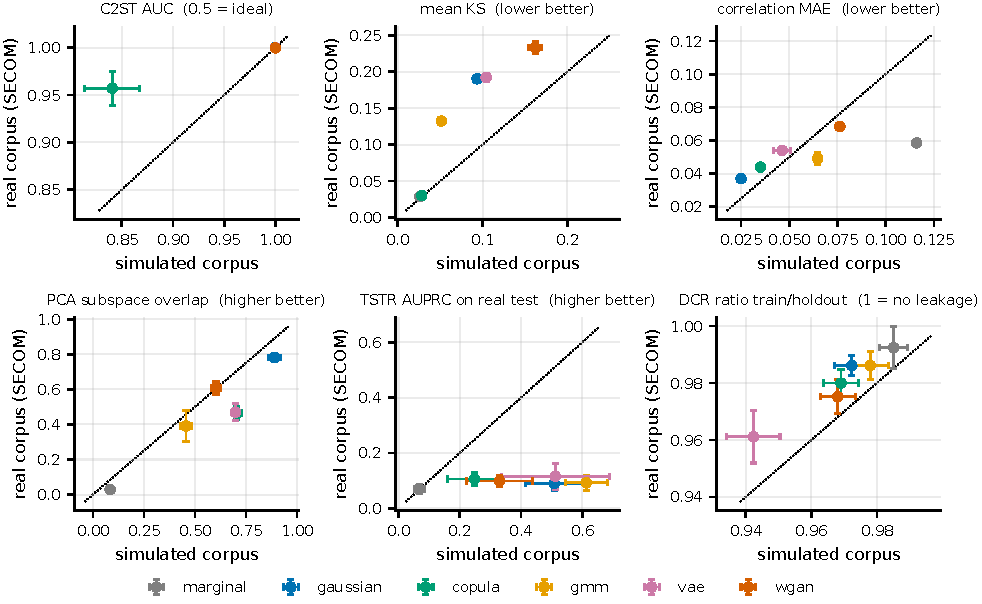
\includegraphics[width=\linewidth]{fig4_cross_corpus.pdf}
\caption{Each panel plots one metric, simulated corpus against real corpus, one
point per generator, error bars are $\pm 1$~sd over \nSeeds{} seeds. The dotted
line is $y=x$. Agreement in \emph{level} would put points on the line;
agreement in \emph{ranking} --- the weaker and more useful property --- would
make the points monotone. Levels differ on every panel. Ranking survives on the
four fidelity and privacy panels and collapses on the two utility panels, which
is the paper's central result in one picture.}
\label{fig:cross}
\end{figure}

\subsection{Generators reproduce the process well and the failures badly}
\label{sec:minority}

The result with the most direct bearing on the application is the simplest. A
synthetic batch-record corpus exists so that people can study batch
\emph{failure}. Table~\ref{tab:main} scores generators on all columns at once,
and on that basis several look respectable. Their reproduction of the failing
class does not match.

On the real corpus, against a true failure rate of \prevReal{}, the variational
autoencoder generates failing records at \sprRatioVaeReal{} times the true rate
and the WGAN at \sprRatioWganReal{} times, while the shrinkage Gaussian generates
them at \sprRatioGaussianReal{} times --- an error of one to two orders of
magnitude in one direction and a fourfold excess in the other. The VAE's deficit
is severe enough that in \vaeDegenRealPct{}\% of seeds it produced too few
failing records to fit a classifier at all, which is why its utility figure rests
on \vaeDegenRealSeeds{} of \nSeeds{} seeds and should not be compared with the
others at face value. The copula and the independence baseline, by contrast,
track the true rate closely (\sprRatioCopulaReal{} and
\sprRatioMarginalReal{} times) --- the latter trivially, since it resamples the
label column on its own.

None of this is visible in the aggregate metrics. A rate error of this size moves
a single column out of several hundred, so mean KS, correlation MAE and C2ST
barely register it. We therefore recommend that the minority-class rate be
reported as a first-class metric in any synthetic manufacturing-data study, and
we note that it is the one metric here that a practitioner could check in a
minute without any of the machinery in this paper.

\subsection{Privacy and the three-way trade-off}

Figure~\ref{fig:tradeoff} places fidelity against privacy on both corpora, with
the bootstrap reference marked. The generators cluster near a DCR ratio of $1$,
consistent with sampling from a learned distribution rather than copying
training records, while bootstrap sits at the degenerate corner. Membership
inference AUC is reported in Table~\ref{tab:main}.

We are careful about what this supports. A DCR ratio near $1$ and a
near-chance distance-based attack are evidence against \emph{crude} memorisation,
and nothing more. Stronger attacks with auxiliary knowledge defeat exactly this
kind of check~\citep{stadler2022synthetic}, and the corpora here contain no
personal data, so these numbers are a methodological demonstration of the third
axis rather than a privacy claim about any deployment. In a real setting the data
at risk would be commercially confidential process knowledge, which has a
different threat model than the individual-record disclosure these metrics were
built for.

\begin{figure}[t]
\centering
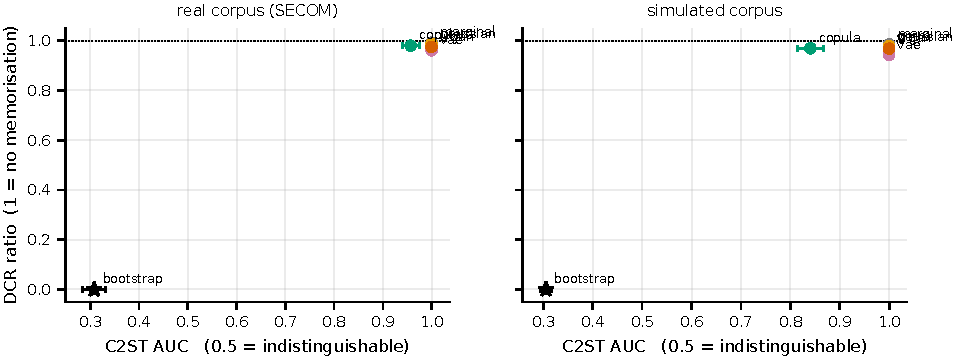
\includegraphics[width=\linewidth]{fig5_tradeoff.pdf}
\caption{Fidelity against privacy, real corpus (left) and simulated corpus
(right). Bootstrap ($\star$) copies training rows: it is the fidelity optimum
and the privacy failure, and it fixes the scale for reading every other point.
Error bars are $\pm1$~sd over \nSeeds{} seeds.}
\label{fig:tradeoff}
\end{figure}

\subsection{Monitoring and release readiness on the simulated corpus}

The monitoring and readiness experiments can only be run on simulated data, since
no real batch trajectories are available to this study. Every number in this
subsection describes the simulator.

We want to be blunt about what that means, because it is the limit of our own
escape from the problem this paper is about. We broke the loop for the tabular
batch-record experiments by bringing in a real corpus. For the trajectory
experiments below we did not, and could not: they are exactly as
self-referential as the practice we criticise in \S\ref{sec:circular}, and
\S\ref{sec:transfer} gives direct evidence that performance measured this way
does not carry over to real process data. The numbers below should be read as a
characterisation of the benchmark, not as an estimate of what a plant would
see.

We use batch-wise unfolded multiway PCA in the Nomikos--MacGregor
tradition~\citep{nomikos1994monitoring,nomikos1995multivariate}: a PCA model is
fitted on nominal training batches, and Hotelling's $T^2$ and squared prediction
error are evaluated on the partial trajectory at 8-hour intervals against limits
calibrated on the nominal reference.

Table~\ref{tab:monitoring} and Figure~\ref{fig:mon} give the operating curve.
Three things are worth stating plainly.

The nominal per-test level does not control the batch-level false-alarm rate. At
a nominal $\alpha = \monAlpha{}$ the realised false-alarm rate on nominal batches
is \monFA{} --- roughly sevenfold --- because two statistics are tested at each
of 28 checkpoints along a batch. Any deployment of this method needs a
multiplicity correction, and reporting the nominal level as if it were the
achieved rate would overstate performance substantially.

At that operating point, failures with a trajectory signature are detected at
\monDetObs{}, with a median time to first alarm of \monTTD{}~h into a
\simDurationH{}-hour batch. Failures without a trajectory signature are detected
at \monDetUnobs{}, which is not distinguishable from the false-alarm rate: the
monitor is not detecting them, it is alarming at its base rate. The two arms rest
on very different denominators --- a test split holds \monNObsFail{} failures
with a signature and only \monNUnobsFail{} without one, which is why the second
figure carries a spread larger than itself. We report it because the argument is
about observability rather than precision, but it should not be read as a
well-estimated rate. No modeling
improvement can change this, because the information is not in the data.

For end-of-production release readiness, a classifier on the trajectory up to
200~h reaches AUROC \readyAUROC{} and AUPRC \readyAUPRC{} against a prevalence
baseline of \readyPrev{}, a lift of \readyLift{}$\times$. That is a real signal on
this simulator. It is also, and only, a statement about this simulator.

\begin{table}[t]
\centering
\footnotesize
\caption{Multiway-PCA monitoring on the simulated corpus, mean\,$\pm$\,sd over
\nSeeds{} seeds. Detection is separated by whether the failure mode leaves a
trajectory signature. The gap between the nominal $\alpha$ and the achieved
false-alarm rate is the multiplicity effect of testing repeatedly along a batch.}
\label{tab:monitoring}
\resizebox{\linewidth}{!}{% AUTO-GENERATED by src/06_tables.py -- do not edit.
\begin{tabular}{rcccc}
\toprule
nominal $\alpha$ & achieved false-alarm rate & detection: signature & detection: none & median TTD (h) \\
\midrule
0.001 & 0.009\,$\pm$\,0.003 & 0.348\,$\pm$\,0.115 & 0.000\,$\pm$\,0.000 & 124\,$\pm$\,47 \\
0.005 & 0.026\,$\pm$\,0.007 & 0.552\,$\pm$\,0.077 & 0.045\,$\pm$\,0.096 & 150\,$\pm$\,18 \\
0.010 & 0.070\,$\pm$\,0.028 & 0.673\,$\pm$\,0.066 & 0.136\,$\pm$\,0.159 & 136\,$\pm$\,11 \\
0.020 & 0.177\,$\pm$\,0.026 & 0.727\,$\pm$\,0.057 & 0.148\,$\pm$\,0.163 & 124\,$\pm$\,11 \\
0.050 & 0.365\,$\pm$\,0.018 & 0.797\,$\pm$\,0.054 & 0.512\,$\pm$\,0.288 & 90\,$\pm$\,16 \\
0.100 & 0.559\,$\pm$\,0.015 & 0.885\,$\pm$\,0.052 & 0.681\,$\pm$\,0.178 & 55\,$\pm$\,14 \\
\bottomrule
\end{tabular}
}
\end{table}

\begin{figure}[t]
\centering
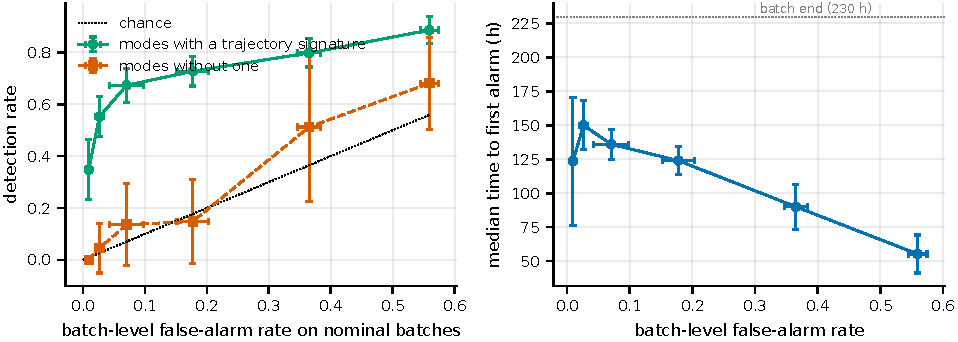
\includegraphics[width=\linewidth]{fig6_monitoring.pdf}
\caption{Left: detection rate against achieved batch-level false-alarm rate,
separately for failure modes with and without a trajectory signature. The
signature-free modes track the chance diagonal --- the monitor is not detecting
them. Right: median time to first alarm; earlier detection is bought entirely
with false alarms.}
\label{fig:mon}
\end{figure}

\section{What this supports, and what stays with the quality unit}
\label{sec:regulatory}

Given the results above, we state the proposed role narrowly.

\paragraph{What is supported.} The \emph{function} a monitor of this kind could
serve is triage: ordering which batch records a reviewer opens first and which
in-process investigations start earlier. We deliberately do not quote our
readiness lift as the expected size of that benefit. It was measured on the
simulator, and \S\ref{sec:transfer} is direct evidence that downstream
performance measured on a simulator does not transfer. What our results support
is that the triage function is worth investigating on real data, and nothing
about how well it would work.

\paragraph{What is not supported, by our own evidence.} Any use in which the
model's output substitutes for, shortens, or provides evidence within the release
decision. Four results forbid it.

Downstream utility conclusions drawn on simulated data do not transfer to real
data ($\rho$~=~\ciAuprcRho{}, with an interval spanning zero; \S\ref{sec:transfer}),
so a
system whose usefulness was established on a simulator has not had its usefulness
established. The prediction task on our simulated corpus is also far easier than the real one
(\trtrAuprcSim{} against \trtrAuprcReal{} at comparable prevalence). We do not
claim that magnitude is general --- it follows from a label our simulator
generates near-deterministically --- and that is the point: a builder with no
real batch records cannot establish whether their simulated task is easier than
the plant's or harder, so a performance figure carried over from simulation
cannot be assumed to describe what the plant would see, in either direction.

A third of the failure modes in our fault model leave no trajectory signature and
are detected at the monitor's base rate, so a ``no alarm'' output carries no
information about whole classes of failure. A negative result that cannot
distinguish absence of fault from absence of observability must never be allowed
to reduce scrutiny --- this is the single most important sentence in this section
for anyone tempted to deploy such a monitor.

And the specification limits themselves are derived from the simulator's own
nominal distribution (\S\ref{sec:sim}), so ``predicting release readiness'' here
means predicting a label the simulator invented.

\paragraph{What stays with the human.} All of it. The disposition decision, the
review of the complete batch record required by \S211.192, the investigation of
any specification failure or unexplained discrepancy, and the certification
signature under Annex~16 remain with the quality control unit and the Qualified
Person respectively~\citep{cfr211,eudralex2015annex16}. A model output is at most
an additional input to a human review that would happen anyway, and its absence
of an alarm must not shorten that review.

\paragraph{The EU is drafting a rule that would exclude this model class
outright.} Annex~22 of EudraLex Volume~4, the GMP annex on artificial
intelligence, is the instrument most directly relevant to everything above. It is
a draft issued for consultation and is \emph{not} in force: the adopted annexes
of Volume~4 run to Annex~21, and Annex~22 is not among
them~\citep{ec2025annex22}. What it proposes matters here anyway, because it is
narrower than the framing of this paper. Its scope covers models "used in
critical applications with direct impact on patient safety, product quality or
data integrity", and it applies only "to static models, i.e.\ models that do not
adapt their performance during use by incorporating new data". Dynamic models
"should not be used in critical GMP applications", and the draft states plainly
that it "does not apply to Generative AI and Large Language Models (LLM), and
such models should not be used in critical GMP applications".

Every generator studied in this paper is a generative model. If Annex~22 is
adopted in anything like its draft form, the model class evaluated here is
excluded from critical GMP applications by rule, independently of how well it
performs. That does not make this work moot --- a benchmark, an evaluation
protocol and a synthetic corpus for research are not critical GMP applications,
and the draft does not reach them. It does mean the honest reading of our results
is narrower still than the transfer result of \S\ref{sec:transfer} already makes
it: not merely that the evidence does not yet support a release-decision role,
but that the regulator with jurisdiction is drafting a rule which would forbid
one for models of this kind. We report this as the current state of a draft, not as settled law.

\paragraph{The qualification path this has not started.} ``Future work''
understates the distance, so rather than name three frameworks we work the
opening steps of one of them through concretely. FDA's draft
credibility-assessment approach for AI supporting regulatory decisions proceeds
through a sequence of steps that begins by defining the question of interest,
then the context of use, then assessing model risk, before any credibility
evidence is planned or gathered~\citep{fda2025aiguidance}. Those first steps are
the only ones a paper without real batch data could discharge, and attempting
them is instructive.

The question of interest is the easy part: \emph{does this batch conform to its
specification?} The context of use is where the exercise breaks. A context of use
has to state which decision the model informs, what else informs that decision,
and what the model does not cover. Written honestly for the system studied here
it reads: a multiway-PCA monitor, trained on synthetic batch records from a
simulator of unestablished realism, ordering the queue in which a reviewer opens
batch records for a process, product and site the model has never seen, with no
coverage of two of the six failure modes in its own fault model and none of any
mode absent from that model. That is narrow to the point of being nearly vacuous,
and writing it down is what makes it obvious --- which is the argument for
drafting a context of use at the start of such a project rather than at its
qualification.

Model risk, in the draft's terms, is a function of how much the model influences
the decision and how severe the consequence of a wrong decision is. Here the
consequence is the most severe the framework contemplates: a non-conforming batch
released to a patient. Influence is therefore the only available lever, and the
triage framing above exists to hold it near zero --- the model changes the
\emph{order} of a review that happens in full regardless, and no model output
shortens, substitutes for, or contributes evidence to the disposition. Severe
consequence with near-zero influence is the only cell of that matrix this system
can occupy today. That is a design constraint rather than a result: any use that
raises influence raises the credibility evidence required with it, to a level
nothing in this paper approaches.

The later steps --- the credibility assessment plan, its execution, the report,
and the determination of adequacy for the context of use --- all require
qualification against \emph{real} batch data from the specific process, product
and site, which does not exist for this system. Alongside them, and under a
risk-based framework such as GAMP~5~\citep{ispe2022gamp5} and
ICH~Q9(R1)~\citep{ich2023q9r1}, a compliant system would need data integrity
controls meeting ALCOA+ over its inputs, change control and revalidation
triggers, drift monitoring with defined action limits, and a documented human
review step the model cannot bypass. This paper contributes to none of them. It
contributes a benchmark on which methods can be compared before any of that
begins, and evidence that the comparisons currently being made are not
informative.

\section{Related work}
\label{sec:related}

\paragraph{Batch process monitoring.} Multiway PCA and PLS for batch
processes~\citep{nomikos1994monitoring,nomikos1995multivariate} remain the
reference method and the baseline we use. Simulation benchmarks in this area ---
PenSim~\citep{birol2002modular} and the industrial-scale
IndPenSim~\citep{goldrick2015development,goldrick2019modern} --- are the
established way to make the field reproducible, and our simulator follows their
kinetic structure. Our disagreement is not with these benchmarks, which are
careful about their own status, but with downstream work that treats performance
on them as evidence about real processes.

\paragraph{Digital twins in pharmaceutical manufacturing.} Reviews of the
area~\citep{chen2020digital} document a rapidly growing literature and, in our
reading, a consistent gap: validation is nearly always against the model's own
simulation or against a single proprietary dataset that cannot be shared. The
regulatory context for advanced manufacturing continues to
develop~\citep{ich2022q13}, which makes the evidentiary standard more, not less,
pressing.

\paragraph{Synthetic tabular data and its evaluation.} CTGAN and
TVAE~\citep{xu2019modeling} defined the modern baselines; sample-level fidelity
metrics~\citep{alaa2022faithful} and the utility-transfer framing used in
healthcare~\citep{rankin2020reliability} shape how such models are assessed.
Work on privacy is the closest in spirit to ours: \citet{stadler2022synthetic}
show that synthetic data does not deliver the privacy guarantees commonly
claimed for it, by testing the claim rather than assuming it. We do the analogous
thing for the fidelity claim in a simulated-benchmark setting. Broader treatments
of what synthetic data is for~\citep{jordon2022synthetic} make the same point we
arrive at empirically: the purpose determines the evaluation, and an evaluation
detached from the purpose is decorative. Generative models for medical time
series~\citep{esteban2017realvalued} face a structurally identical problem.

\section{Limitations}
\label{sec:limitations}

We list these in descending order of how much they should reduce confidence in
the paper's claims.

\paragraph{The real corpus is not pharmaceutical.} \corpusreal{} is semiconductor
manufacturing. It has the structure our protocol needs --- real, high-dimensional
process data with a rare, genuine disposition label --- but the transfer result
in \S\ref{sec:transfer} is, strictly, about transfer from our fermentation
simulator to a semiconductor process. A defender of simulator-based validation
can reasonably answer that a pharmaceutically faithful simulator would transfer
better to a pharmaceutical corpus. We cannot rule that out, and no public data
lets us test it. What the result does establish is that agreement between a
simulator and real process data is not automatic and must be demonstrated rather
than assumed. Obtaining even one real batch-record corpus, under any access
arrangement, would be worth more than any methodological improvement in this
paper. We tried for a closer substitute and did not get one: the IndPenSim
100-batch dataset~\citep{goldrick2019indpensim} would have supplied
pharma-relevant batch and phase structure, and it is not part of this study. It
is also itself a simulation, so it would have narrowed the gap rather than
closed it.

\paragraph{The simulator is not calibrated.} Its structure follows published
fed-batch models but its parameters were not fitted to plant data and its
absolute product scale is arbitrary. Specification limits are consequently
derived from its own nominal distribution (\S\ref{sec:sim}). Every monitoring and
readiness number in \S\ref{sec:results} inherits this and describes the simulator
only.

\paragraph{\nMethods{} methods is a weak ranking test.} Every correlation is a
Spearman coefficient over six points. Computing it per seed gives \nSeeds{}
estimates and an interval, which is what we report, but it does not create
information about methods we did not run: a seventh generator could sit anywhere.
A larger and more diverse generator set would sharpen this. The per-seed
estimates within a metric also share those six methods, so the Mann--Whitney
contrast in \S\ref{sec:transfer} is descriptive rather than confirmatory.

\paragraph{The difficulty gap may be a property of our simulator, not of
simulators.} Our headline observation that the simulated task is far easier than
the real one (\trtrAuprcSim{} against \trtrAuprcReal{}) could be read as a
criticism of this particular simulator: perhaps a harder one would close the gap.
We think that reading strengthens rather than weakens the paper's point, since
nobody building a simulator without real batch records can know where on that
difficulty scale they have landed --- but it does mean the specific magnitude of
the gap is not a general constant, and we do not present it as one.

\paragraph{The VAE's utility figure is not comparable.} It rests on
\vaeDegenRealSeeds{} of \nSeeds{} seeds because the model failed to generate
enough failing records in the rest (\S\ref{sec:minority}). We report it in
Table~\ref{tab:main} for completeness and exclude it from any claim about which
method is best on real data.

\paragraph{The generators are re-implementations.} We implement a WGAN-GP rather
than running CTGAN itself, and a plain MLP VAE rather than TVAE. The families are
represented; the specific published architectures and their tuned
hyperparameters are not, and a generative-modeling reviewer would be right to
want the reference implementations. Neural generators were trained with a fixed
budget and no per-corpus hyperparameter search, which plausibly disadvantages
them relative to the closed-form models.

\paragraph{The failure-mode prior is biased by construction.} Recall records
count escapes, not rejections. Modes that release reliably catches are
under-represented in our prior, which means the simulator's fault mix is skewed
toward the failures that get through --- arguably the wrong direction for a
benchmark about detection.

\paragraph{We did not test whether the empirical prior changes anything.} The
abstract and \S\ref{sec:anchors} lead with the recall corpus as the study's
anchor to real data, and it does real work in one narrow sense: it fixes the
relative frequency of six failure modes. It does not fix the absolute failure
rate, the fault magnitudes, or the specification limits, all of which are assumed
or self-derived. The obvious control --- regenerate the corpus with a uniform
failure-mode prior and see which conclusions move --- was not run. Until it is,
the influence of the anchoring on any reported result is unquantified, and the
prominence we give it in the framing is not yet earned.

\paragraph{Privacy results are a demonstration, not a guarantee.} Distance-based
membership inference is a weak attack, the corpora contain no personal data, and
the confidentiality interest in real batch records is commercial process
knowledge rather than individual records. Nothing here licenses a privacy claim
about a deployed system.

\paragraph{Monitoring uses one method family.} Multiway PCA is the reference
baseline, not the state of the art. A recurrent or attention-based detector might
do better on the observable modes; it could not do better on the unobservable
ones, which is where the ceiling lies.

\section{Conclusion}

Synthetic digital twins of pharmaceutical manufacturing are usually validated
against the simulators that produced their training data. Running one identical
evaluation protocol on a simulated corpus and on a real manufacturing corpus, we
find that this practice is sound for some questions and empty for the one that
matters. Fidelity and privacy rankings transfer well
($\rho \in [\ciFidPrivLo{}, \ciFidPrivHi{}]$ over \agreeFidPrivN{} metrics),
which is more than we expected. Downstream utility rankings do not
($\rho$~=~\ciAurocRho{} and $\rho$~=~\ciAuprcRho{}; both intervals span zero),
and the prediction
task on our simulated corpus is so much easier than the real one
(\trtrAuprcSim{} against \trtrAuprcReal{}) that absolute performance measured on
it cannot be carried across at all --- a gap that belongs to this simulator's
near-deterministic disposition label rather than to simulators in general, and
whose size and sign a builder without real batch records has no way to check. Alongside this, generators misestimate the failing-batch rate by
one to two orders of magnitude without their aggregate scores reflecting it, and
trajectory monitoring has a hard ceiling set by failure modes the instrumentation
cannot see.

The practical reading is narrow and, we think, actionable: a simulator is an
acceptable venue for asking whether a generative model has learned a
distribution, and is not evidence of anything about whether the resulting
synthetic data is useful. We offer the benchmark, the protocol and the negative
results as a starting point rather than a solution, and we are explicit that none
of it belongs near a release decision. Batch release is a human act with a named
owner and a legal consequence; the contribution available to modeling work here
is to make the evidence for such systems checkable, which begins with declining
to score them against themselves.

\section*{Reproducibility}

All results are produced by the scripts in \texttt{src/}, run in order:
\texttt{01\_profile\_real\_data.py} profiles the real anchors,
\texttt{02\_simulator.py} generates the simulated corpus,
\texttt{03\_evaluate.py} runs the generator protocol on both corpora,
\texttt{04\_monitoring.py} runs the trajectory experiments,
\texttt{05\_figures.py} draws every figure, \texttt{06\_tables.py} emits
\texttt{numbers.tex} and the three \texttt{table\_*.tex} files,
\texttt{07\_agreement\_ci.py} computes the per-seed rank correlations, their
intervals and the fidelity-versus-utility contrast, and
\texttt{08\_verify\_manuscript.py} re-checks the manuscript against the recorded
results. Every numeral in this paper is a
macro defined in \texttt{numbers.tex} and read from a JSON file in
\texttt{results/}; none is typed by hand. Seeds, library versions and the
platform are recorded in each results file. All stochastic results use the same
ten seeds. Claude (Anthropic) was used to assist in developing and revising the
code in \texttt{src/}; every script was read, executed and validated by the
author, and the recorded results files are the output of those validated runs.

\section*{Data availability}

SECOM is available from the UCI Machine Learning Repository under a Creative
Commons Attribution 4.0 International license, which permits reuse with
attribution~\citep{mccann2008secom}; we use it unmodified and redistribute no
part of it. The openFDA drug enforcement export is in the public
domain~\citep{openfda2026enforcement}; the export used here is dated
\recallExport{}, recorded in \texttt{results/failure\_mode\_prior.json}. The
simulated corpus is not distributed because it does not need to be: script~02
regenerates it bit-for-bit from the master seed recorded in
\texttt{results/simulator\_spec.json}.
No proprietary, confidential or internal data of any organization was used.

\section*{Code availability}

All code, the recorded results files and the figure sources are available at
\url{https://github.com/phanibalagam/circular-by-construction} and archived at
\url{https://doi.org/10.5281/zenodo.22855260}, which resolves to the current
version. Running the eight numbered scripts in \texttt{src/} in order reproduces
every number and every figure in this paper from the two public datasets named
above.

\section*{CRediT authorship contribution statement}

\textbf{Phani Kumar Balagam:} Conceptualization, Methodology, Software,
Validation, Formal analysis, Investigation, Data curation, Writing --- original
draft, Writing --- review and editing, Visualization, Project administration.
Sole author; no funding was received and no other person contributed to this
work.

\appendix

\section{Simulator calibration record}
\label{app:calibration}

\S\ref{sec:results} discloses that the simulator was calibrated before any
evaluation was run. This appendix records the sequence, because a paper about
undisclosed evaluation choices should let a reader audit its own. Nothing here is
a result; all of it is modeling history.

\paragraph{What was set, and from where.} Seventeen process parameters carry a
nominal value and a batch-to-batch coefficient of variation, each tagged in
\texttt{src/02\_simulator.py} with the quantity it represents --- Monod
half-saturation constants for substrate and dissolved oxygen, biomass and product
yields, specific production rate, substrate inhibition of production, biomass
decay, maintenance, product hydrolysis, oxygen transfer, feed and initial
substrate concentrations, working volume and inoculum density. The coefficients
of variation range from 0.02 (working volume) to 0.20 (inoculum density), the
latter standing for seed-train variability. Nominal values sit in the ranges
reported for the fed-batch penicillin model family this structure is taken from.
None was fitted to data, from any plant, at any point.

\paragraph{The passes that were run.} Kinetic parameters and the exponential feed
profile were adjusted over several passes until two properties held: batches
completed the production phase without exhausting substrate or oxygen, and the
nominal titer distribution was unimodal with a spread that left a non-trivial
fraction of batches near any plausible lower limit. Neither criterion refers to
real data; both are internal consistency checks on the model. The number of
passes was not logged, which is itself a limitation of this record.

\paragraph{The specification limits were changed once, and it mattered.} Limits
were first asserted as fixed values chosen to look like product specifications.
Against the simulator's own nominal output those values rejected every batch,
which established only that the model's absolute scales --- titer above all ---
are arbitrary. They were replaced with percentiles of the simulator's own
nominal, fault-free distribution: the \simSpecPercentile{}th percentile in each
tail, the $\pm 3\sigma$ equivalent for a normal, estimated over
\simSpecCalBatches{} fault-free batches drawn on a random stream separate from
the one that generates the study corpus. The discarded asserted values are not
recorded and we do not reconstruct them. The consequence is stated where it
matters rather than only here: a label defined by percentiles of the simulator's
own output means ``predicting release readiness'' on this corpus is predicting a
label the simulator invented (\S\ref{sec:regulatory}), and every monitoring and
readiness number inherits it (\S\ref{sec:limitations}).

\paragraph{The failure rate is an assumption, not an estimate.} The nominal batch
failure rate was set to match \corpusreal{}'s observed rate so the two corpora
are comparable in class balance. It was not taken from the recall corpus: recall
records count market escapes, not batch rejections, and cannot estimate a
rejection rate. The recall corpus fixes only the \emph{relative} frequency of the
six retained failure modes, after five openFDA categories were excluded with the
reason for each recorded in the source. Fault magnitudes are hand-chosen uniform
ranges. \S\ref{sec:limitations} states that the control for this --- regenerating
the corpus under a uniform failure-mode prior --- was not run.

\paragraph{What was fixed in advance and not revisited.} The master seed, the
ten evaluation seeds, the generator set, the metric set, the four process phases,
the eight release CQAs, the six-mode fault model and the two-of-six observability
ceiling were all set before the evaluation and not changed after results arrived.
The one budget change after that point is disclosed in \S\ref{sec:results}: the
neural and classifier-two-sample-test budgets were cut once for runtime, before
the reported runs, and applied uniformly thereafter.

\section*{Declaration of generative AI and AI-assisted technologies in the
manuscript preparation process}

During the preparation of this work the author used Claude (Anthropic) in order
to support the drafting and editing of manuscript text and the development and
revision of analysis code. After using this tool, the author reviewed and edited
the content as needed and takes full responsibility for the content of the
published article. The author retained sole responsibility for all final
decisions concerning the research question, study design, data selection, outcome
definitions, analytical methods and experimental controls; independently verified
all sources, data and results; executed and validated the analyses; and
interpreted the findings. No AI tool is listed as an author of this work, and
none could be: authorship carries accountability that no tool can hold.

\bibliographystyle{plainnat}
\bibliography{references}

\end{document}
